\chapter{Evaluation}
\label{chap:evaluation}
In this chapter, our objective is to assess and examine the existing search engine implementation. The evaluation process is structured into three primary segments: Crawler, Indexer, and User Experience.

\section{Testing Environment}
The evaluation procedure is significantly influenced by the specific computing device executing the tests. Displaying information about the testing machine utilized can provide enhanced clarity and facilitate meaningful comparisons.


\begin{table}[ht] 
{\footnotesize
\begin{tabular}{ P{2.5cm} ||P{11.1cm}  }      % centered columns (3 columns) 
 \hline \hline
\textbf{Operating System} & Ubuntu 22.04.3 LTS \T\B 
\\ 
\hline
\textbf{CPU} & Intel(R) Core(TM) i7-10510U @ 1.80GHz; 4 cores; 8 threads \T\B 
\\ 
\hline
\textbf{RAM} & 32GB\T\B 
\\ 
\hline
\textbf{Machine} & Lenovo ThinkPad P15s Gen 1\T\B 
\\ 
\hline \hline
    \end{tabular}
}
  \captionsetup{justification=centering,margin=2cm}
  \caption{Local machine setup}
\end{table}

\section{Crawler}  

To evaluate the web crawler, the following criteria can be employed for measurement:


{\renewcommand\labelitemi{}
\begin{itemize}
  \item \textbf{Coverage}: This metric measures the proportion of relevant web pages that the crawler can locate and fetch from the internet.

  \item \textbf{Scalability}: It evaluates the crawler's facility for efficiently scaling up to add more computing power to crawl more content.

  \item \textbf{Versatility}: Can the crawler be applied to explore diverse types of content from various websites, encompassing text, multimedia, and links?

  \item \textbf{Robustness}: The crawler's ability to adeptly manage challenging scenarios and errors.

  \item \textbf{Politeness}:  the extent to which the crawler respects the rules and policies of the web servers and avoids overloading them with requests and forbidden links.

\end{itemize}

\subsection{Datasets} 
Evaluating a web crawler necessitates the utilization of a static website as a reliable reference point. The crawler-test\footnote{\url{https://crawler-test.com/}} website serves as an excellent choice for this purpose due to its diverse range of content and links, containing a wide range of scenarios that a crawler might encounter. This website effectively employs robots.txt to provide guidance to the crawler, allowing for an assessment of its politeness. Moreover, it includes a section containing links that yield various HTTP request status codes, such as 4xx and 5xx, which proves valuable for ensuring the crawler's robustness. Additionally, it incorporates multiple instances of page redirection, including scenarios like infinite redirection, which serves the dual purpose of evaluating the crawler's ability to avoid traps and enhancing its overall resilience.

To enhance the coverage and versatility of our crawler testing, we are considering two additional websites encompassing a broader range of use cases, ensuring that the crawler can effectively handle various HTML structures and more generic scenarios.
The first use case involves extracting product information from an E-commerce platform like Douglas\footnote{\url{https://www.douglas.de/}}. This website offers over 160,000 diverse products, making it an ideal candidate for testing different content types, including images. We will categorize our testing into three distinct datasets: small (with 100 products), medium (with 1,000 products), and large (with 10,000 products) to evaluate the crawler's performance under different data sizes thoroughly.
The second website, Times Higher Education\footnote{\url{https://www.timeshighereducation.com/world-university-rankings/2023/world-ranking}}, specializes in annually ranking universities. This unique characteristic allows us to evaluate content changes occurring on a yearly basis, setting it apart from other websites that undergo daily alterations, which can prove challenging for accurate evaluation.

\subsection{Experiments}
The crawler-test website is selected to assess and experiment with various crawler configurations. This choice is attributed to its stable, non-changing nature, which facilitates straightforward and meaningful comparisons of results across different configurations.
 
The first testing case is the coverage. It is vital to ensure the crawler can find the links inside the page, navigate to them and crawl them. 

\begin{table}[ht] 
{\footnotesize
\begin{tabular}{ P{3cm} ||P{10.1cm}  }      % centered columns (3 columns) 
 \hline \hline
\textbf{Seed URL} & \href{https://crawler-test.com/}{https://crawler-test.com/}\T\B 
\\ 
\hline
\textbf{Allow Multi Elements} & False \T\B 
\\ 
\hline
\textbf{Max Pages} & 1000\T\B 
\\ 
\hline
\textbf{Threads} & 1\T\B 
\\ 
\hline
\textbf{Max Depth} & 1\T\B 
\\ 
\hline
\textbf{Pagination} & None\T\B 
\\ 
\hline
\textbf{Actions} & None\T\B 
\\ 
\hline
\textbf{Inspectors} & //*[contains(@class, 'large-12 columns')]\T\B 
\\ 
\hline
\textbf{Max Docs} & 1000\T\B 
\\ 
\hline \hline
    \end{tabular}
}
  \captionsetup{justification=centering,margin=2cm}
  \caption{Crawler configuration}
\end{table}



\begin{table}[ht] 
{\footnotesize
\begin{tabular}{ P{3cm} ||P{10.1cm}  }      % centered columns (3 columns) 
 \hline \hline
\textbf{Links} & Collected: 406/415 . Visited Correctly: 402. Cross Site: 6 . Already Visited: 0\T\B 
\\ 
\hline
\textbf{Time} & Tot. Spent: 671.19 s. Avg. Processing: 1.98 s. Avg. Page Loading: 0.697 s\T\B 
\\
\hline
\textbf{Status Codes} &   101: 1  102: 1  200: 321  201: 1  202: 1  203: 1  206: 3  207: 1  226: 1  300: 1  305: 2  306: 1  400: 1  401: 1  402: 1  403: 2  404: 11  405: 1  406: 1  407: 1  408: 1  409: 1  410: 1  411: 1  412: 1  413: 1  414: 1  415: 1  416: 1  417: 1  418: 1  419: 1  420: 1  421: 1  422: 1  423: 1  424: 1  426: 1  428: 1  429: 1  431: 1  440: 1  444: 1  449: 1  450: 1  451: 1  494: 1  495: 1  496: 1  497: 1  498: 1  499: 1  500: 2  501: 1  502: 1  503: 1  504: 1  505: 1  506: 1  507: 1  508: 1  509: 1  510: 1  511: 1  520: 1  598: 1  
599: 1\T\B 
\\ 
\hline
\textbf{Docs \& Content} & Tot. Docs Found: 255. Duplicated Content:24. Avg. Docs Per Page:1. Average page size: 0.000346\T\B 
\\ 
\hline
\textbf{Robots.txt Exists} & True\T\B 
\\ 
\hline
\textbf{Tot. Errors} & 6\T\B 
\\ 
\hline \hline
    \end{tabular}
}
  \captionsetup{justification=centering,margin=2cm}
  \caption{Crawler configuration}
\end{table}

Checking if changing thew depth will increase the coverage.


\begin{table}[ht] 
{\footnotesize
\begin{tabular}{ P{3cm} ||P{10.1cm}  }      % centered columns (3 columns) 
 \hline \hline
\textbf{Seed URL} & \href{https://crawler-test.com/}{https://crawler-test.com/}\T\B 
\\ 
\hline
\textbf{Allow Multi Elements} & False \T\B 
\\ 
\hline
\textbf{Max Pages} & 1000\T\B 
\\ 
\hline
\textbf{Threads} & 1\T\B 
\\ 
\hline
\textbf{Max Depth} & 10\T\B 
\\ 
\hline
\textbf{Pagination} & None\T\B 
\\ 
\hline
\textbf{Actions} & None\T\B 
\\ 
\hline
\textbf{Inspectors} & //*[contains(@class, 'large-12 columns')]\T\B 
\\ 
\hline
\textbf{Max Docs} & 1000\T\B 
\\ 
\hline \hline
    \end{tabular}
}
  \captionsetup{justification=centering,margin=2cm}
  \caption{Crawler configuration}
\end{table}



\begin{table}[ht] 
{\footnotesize
\begin{tabular}{ P{3cm} ||P{10.1cm}  }      % centered columns (3 columns) 
 \hline \hline
\textbf{Links} & Collected: 895 . Visited Correctly: 697. Cross Site: 198 . Already Visited: 0. Excluded: 1\T\B 
\\ 
\hline
\textbf{Time} & Tot. Spent: 760.84 s. Avg. Processing: 3.26 s. Avg. Page Loading: 1.03 s\T\B 
\\
\hline
\textbf{Status Codes} &     101: 1  102: 1  200: 220  201: 1  202: 1  203: 1  206: 3  207: 1  226: 1  300: 1  305: 2  306: 1  400: 1  401: 1  402: 1  403: 2  404: 7  405: 1  406: 1  407: 1  408: 1  409: 1  410: 1  411: 1  412: 1  413: 1  414: 1  415: 1  416: 1  417: 1  418: 1  419: 1  420: 1  421: 1  422: 1  423: 1  424: 1  426: 1  428: 1  429: 1  431: 1  440: 1  444: 1  449: 1  450: 1  451: 1  494: 1  495: 1  496: 1  497: 1  498: 1  499: 1  500: 2  501: 1  502: 1  503: 1  504: 1  505: 1  506: 1  507: 1  508: 1  509: 1  510: 1  511: 1  520: 1  598: 1  
599: 1\T\B 
\\ 
\hline
\textbf{Docs \& Content} & Tot. Docs Found: 375. Duplicated Content: 667. Avg. Docs Per Page:1. Average page size: 0.0562\T\B 
\\ 
\hline
\textbf{Robots.txt Exists} & True\T\B 
\\ 
\hline
\textbf{Tot. Errors} & 21\T\B 
\\ 
\hline \hline
    \end{tabular}
}
  \captionsetup{justification=centering,margin=2cm}
  \caption{Crawler configuration}
\end{table}


Multi threading


\begin{table}[ht] 
{\footnotesize
\begin{tabular}{ P{3cm} ||P{10.1cm}  }      % centered columns (3 columns) 
 \hline \hline
\textbf{Seed URL} & \href{https://crawler-test.com/}{https://crawler-test.com/}\T\B 
\\ 
\hline
\textbf{Allow Multi Elements} & False \T\B 
\\ 
\hline
\textbf{Max Pages} & 1000\T\B 
\\ 
\hline
\textbf{Threads} & 4\T\B 
\\ 
\hline
\textbf{Max Depth} & 10\T\B 
\\ 
\hline
\textbf{Pagination} & None\T\B 
\\ 
\hline
\textbf{Actions} & None\T\B 
\\ 
\hline
\textbf{Inspectors} & //*[contains(@class, 'large-12 columns')]\T\B 
\\ 
\hline
\textbf{Max Docs} & 1000\T\B 
\\ 
\hline \hline
    \end{tabular}
}
  \captionsetup{justification=centering,margin=2cm}
  \caption{Crawler configuration}
\end{table}



\begin{table}[ht] 
{\footnotesize
\begin{tabular}{ P{3cm} ||P{10.1cm}  }      % centered columns (3 columns) 
 \hline \hline
\textbf{Links} & Collected: 895 . Visited Correctly: 697. Cross Site: 199 . Already Visited: 227. Excluded: 1\T\B 
\\ 
\hline
\textbf{Time} & Tot. Spent: 760.84 s. Avg. Processing: 3.26 s. Avg. Page Loading: 1.03 s\T\B 
\\
\hline
\textbf{Status Codes} &     101: 2, 102: 2, 200: 823, 201: 2, 202: 2, 203: 2, 204: 1, 206: 5, 207: 2, 226: 2, 300: 2, 305: 4, 306: 2, 400: 2, 401: 2, 402: 2, 403: 4, 404: 66, 405: 2, 406: 2, 407: 2, 408: 2, 409: 2, 410: 2, 411: 2, 412: 2, 413: 2, 414: 2, 415: 2, 416: 2, 417: 2, 418: 2, 419: 2, 420: 2, 421: 2, 422: 2, 423: 2, 424: 2, 426: 2, 428: 2, 429: 2, 431: 2, 440: 2, 444: 2, 449: 2, 450: 2, 451: 2, 494: 2, 495: 2, 496: 2, 497: 2, 498: 2, 499: 2, 500: 4, 501: 2, 502: 2, 503: 2, 504: 2, 505: 2, 506: 2, 507: 2, 508: 2, 509: 2, 510: 2, 511: 2, 520: 2, 598: 2, 599: 2\T\B 
\\ 
\hline
\textbf{Docs \& Content} & Tot. Docs Found: 533. Duplicated Content: 333. Avg. Docs Per Page:1. Average page size: 0.0562\T\B 
\\ 
\hline
\textbf{Robots.txt Exists} & True\T\B 
\\ 
\hline
\textbf{Tot. Errors} & 21\T\B 
\\ 
\hline \hline
    \end{tabular}
}
  \captionsetup{justification=centering,margin=2cm}
  \caption{Crawler configuration}
\end{table}


Comparing threads impact

\begin{figure}[h]	
     \centering
     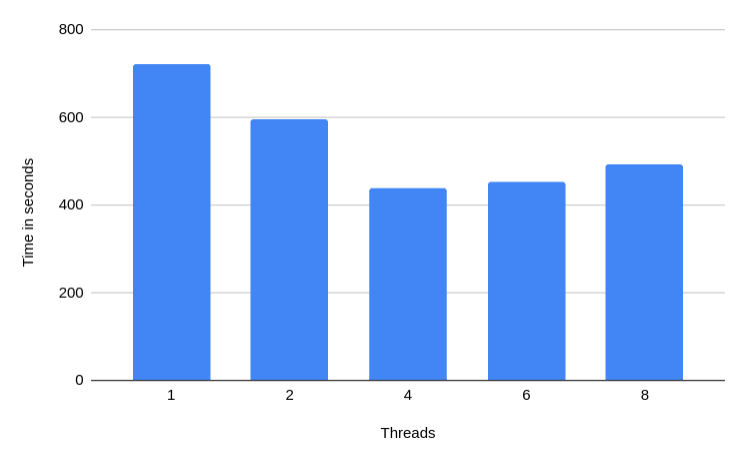
\includegraphics[width=13cm]{images/threads-table.png}
     \caption{Comparing threads performance.}
     \label{fig:google-arch}
\end{figure}

Threads docs sharing

\begin{figure}[h]	
     \centering
     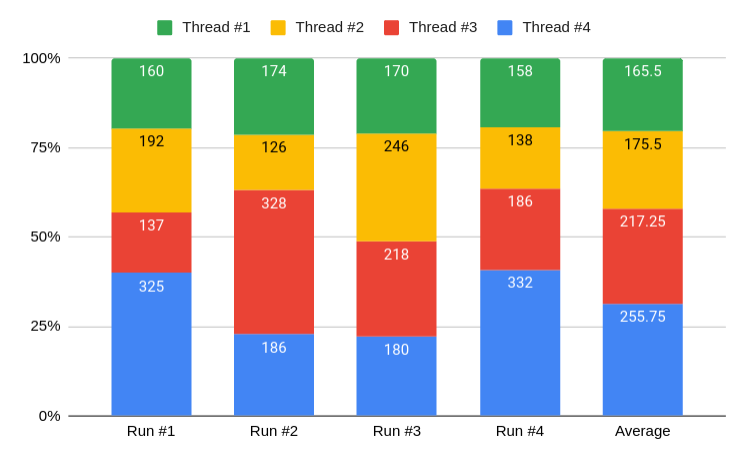
\includegraphics[width=13cm]{images/threads_share.png}
     \caption{Threads documents distribution.}
     \label{fig:google-arch}
\end{figure}

Testing other different sites: 

\begin{table}[ht] 
{\footnotesize
\begin{tabular}{ P{3cm} ||P{10.1cm}  }      % centered columns (3 columns) 
 \hline \hline
\textbf{Seed URL} & \href{https://www.timeshighereducation.com/world-university-rankings/2023/world-ranking}{https://www.timeshighereducation.com/world-university-rankings/2023/world-ranking}\T\B 
\\ 
\hline
\textbf{Allow Multi Elements} & False \T\B 
\\ 
\hline
\textbf{Max Pages} & 100\T\B 
\\ 
\hline
\textbf{Threads} & 1\T\B 
\\ 
\hline
\textbf{Max Depth} & 100\T\B 
\\ 
\hline
\textbf{Pagination} & //*[contains(@class, 'pagination')]\T\B 
\\ 
\hline
\textbf{Actions} & None\T\B 
\\ 
\hline
\textbf{Inspectors} & //*[contains(@class, 'ranking-institution-title')] \newline //*[contains(concat(' ', normalize-space(@class), ' '), ' location ')] \newline //*[contains(@class, 'rank') and contains(@class, 'sorting\_1') and contains(@class, 'sorting\_2')]
\T\B 
\\ 
\hline
\textbf{Max Docs} & 1000\T\B 
\\ 
\hline \hline
    \end{tabular}
}
  \captionsetup{justification=centering,margin=2cm}
  \caption{Crawler configuration}
\end{table}



\begin{table}[ht] 
{\footnotesize
\begin{tabular}{ P{2.5cm} ||P{11.1cm}  }      % centered columns (3 columns) 
 \hline \hline
\textbf{Links} & 
\begin{tabular}{c|c|c|c|c}
       Collected   & Visited Correctly & Already Visited & Cross Site &  Excluded\T\B \\\hline
       95/95 & 95 & 0 & 0 & 1
\end{tabular}
\\ 
\hline
\textbf{Time} &
\begin{tabular}{P{3cm}|P{3cm}|P{3cm}}
       Tot. Spent & Avg. Processing & Avg. Page Loading \T\B \\\hline
       395.209 s & 3.16 s & 1.26 s 
\end{tabular}
\\
\hline
\textbf{Status Codes} &     403: 95\T\B 
\\ 
\hline
\textbf{Docs \& Content} & 
\begin{tabular}{c|c|c|c}
       Tot. Docs   & Duplicated Content & Avg. Docs Per Page & Avg. Page Size\T\B \\\hline
       2389 & 0 & 25 & 0.2227
\end{tabular}
\\ 
\hline
\textbf{Robots.txt Exists} & True\T\B 
\\ 
\hline
\textbf{Tot. Errors} & 1\T\B 
\\ 
\hline \hline
    \end{tabular}
}
  \captionsetup{justification=centering,margin=2cm}
  \caption{Crawler configuration}
\end{table}


Douglas Use case:


\begin{table}[ht] 
{\footnotesize
\begin{tabular}{ P{3cm} ||P{10.1cm}  }      % centered columns (3 columns) 
 \hline \hline
\textbf{Seed URL} & \href{https://www.douglas.de/de/c/parfum/damenduefte/duftsets/010111}{https://www.douglas.de/de/c/parfum/damenduefte/duftsets/010111}\T\B 
\\ 
\hline
\textbf{Allow Multi Elements} & False \T\B 
\\ 
\hline
\textbf{Max Pages} & 1000\T\B 
\\ 
\hline
\textbf{Threads} & 4\T\B 
\\ 
\hline
\textbf{Max Depth} & 10\T\B 
\\ 
\hline
\textbf{Pagination} & //*[contains(@class, 'pagination')]\T\B 
\\ 
\hline
\textbf{Actions} & None\T\B 
\\ 
\hline
\textbf{Inspectors} & //*[contains(@class, 'header-name')]\T\B  \newline
//*[contains(@class, 'product-price\_\_price')][1] \newline
//*[contains(@class, 'zoom-image')]/img \newline
//*[contains(@class, 'third-line')] 
\\ 
\hline
\textbf{Max Docs} & 1000\T\B 
\\ 
\hline \hline
    \end{tabular}
}
  \captionsetup{justification=centering,margin=2cm}
  \caption{Crawler configuration}
\end{table}



\begin{table}[ht] 
{\footnotesize
\begin{tabular}{ P{2.5cm} ||P{11.1cm}  }      % centered columns (3 columns) 
 \hline \hline
\textbf{Links} & 
\begin{tabular}{c|c|c|c|c}
       Collected   & Visited Correctly & Already Visited & Cross Site &  Excluded\T\B \\\hline
       8/8 & 8 & 0 & 0 & 0
\end{tabular}
\\ 
\hline
\textbf{Time} &
\begin{tabular}{P{3cm}|P{3cm}|P{3cm}}
       Tot. Spent & Avg. Processing & Avg. Page Loading \T\B \\\hline
       395.209 s & 7.87 s & 2.638 s 
\end{tabular}
\\
\hline
\textbf{Status Codes} &     200: 8\T\B 
\\ 
\hline
\textbf{Docs \& Content} & 
\begin{tabular}{c|c|c|c}
       Tot. Docs   & Duplicated Content & Avg. Docs Per Page & Avg. Page Size\T\B \\\hline
       245 & 0 & 49 & 1.509
\end{tabular}
\\ 
\hline
\textbf{Robots.txt Exists} & True\T\B 
\\ 
\hline
\textbf{Tot. Errors} & 0\T\B 
\\ 
\hline \hline
    \end{tabular}
}
  \captionsetup{justification=centering,margin=2cm}
  \caption{Crawler configuration}
\end{table}

\section{Indexer}  
\section{User Experience} 
 